\documentclass[a4paper, 12pt]{article}
\usepackage[ngerman]{babel}
\usepackage[utf8]{inputenc}
\usepackage{amsmath}
\usepackage{amsfonts}
\usepackage{listings}
\usepackage{pgfplots}
\usepackage{graphicx}
\pgfplotsset{compat=1.9}
\usepackage{tikz}
\usepackage{float}
\author{Autor \\ Lukas Hofmaier \and Betreuer\\ Prof. Hansjörg Huser \\}
\title{Recommender System basierend auf Haskell \\ \vspace{2 mm} {\large Ein Report zu Userbased Collaborative Filtering und Matrixfaktorisierung}}
\date{
\textsc{University of Applied Science Rapperswil}\\
Projektarbeit \\ \today
}

\begin{document}

\lstset{basicstyle=\small,
language=Haskell,
stringstyle=ttfamiliy
}

\maketitle
\newpage
\tableofcontents
\newpage
\begin{abstract}
Recommender nutzen Datenbanken mit Pr"aferenzen von Kunden, um ihnen aus einer grossen Auswahl von Artikel diejenigen zu empfehlen, die sie interessieren k"onnten. Collaborative Filtering ist eine Klasse von Recommender, die Empfehlungen aufgrund von Verhaltensmuster anderer User berechnen.
In diesem Report werden zwei Collaborative Filtering Methoden beschrieben. Userbased Collaborative Filtering ist eine der ersten und intuitivsten Methoden. Matrixfaktorisierung ist eine weitere Methode, die an der Netflix Competition die besten Resultate lieferte.

Die Algorithmen werden mit einer geeigneten Evaluation verglichen. Die Evaluation und die Algorithmen wurden in Haskell implementiert.

\end{abstract}

\section{Recommender-Problem}
\label{sec:problem}
Dieser Abschnitt beschreibt, was ein Recommendersystem ist und weshalb es einen Mehrwert schaffen kann.

Konsumenten werden heute in vielen Bereichen mit einer un"uberschaubaren Anzahl an Kaufm"oglichkeiten konfrontiert. In einem Webshop f"ur B"ucher oder Filme ist es f"ur den Konsumenten beispielsweise schwierig, alle Artikel im Angebot anzuschauen und aufgrund dieser Evaluation die besten Artikel auszuw"ahlen. Beim Recommender-Problem geht es darum aus einer Menge von Artikel (Items) ein sortierte Liste mit den empfehlenswertesten Artikel f"ur einen spezifischen Kunden (User) zu erstellen. Recommender kommen vorallem dort zum Einsatz, wo pers"onlicher Geschmack bei der Bewertung von Artikel eine wichtige Rolle spielt.

Ein Recommendersystem kann eine Bewertung absch"atzen (vorhersagen), die ein bestimmter User einem bestimmten Item gibt. Recommender berechnen die Bewertungen f"ur Items, die der User noch nicht gesehen hat. Die Items mit den besten Bewertungen werden dem User empfohlen.

Recommendersysteme werden vorallem im e-Commerce eingesetzt. Man kann sie aber auch dazu verwenden, um unwichtige Informationen von wichtigen zu trennen. Recommender k"onnen beispielsweise auch f"ur Information Retrieval eingesetzt werden. Sie generieren eine Liste von Dokumenten die der User noch nicht gesehen hat \cite{herlocker00}.

In nachfolgenden Text wird haupts"achlich von User und Items gesprochen. Sie sind folgendermassen definiert.

\begin{description}
\item[User] User sind die Konsumenten. F"ur sie berechnet das Recommendersystem Empfehlungen. 
User haben Pr"aferenzen und bewerten Items aufgrund des pers"onlichen Geschmacks. In einer Information Retrieval Anwendung k"onnen User auch einfach die Benutzer der Software sein.
\item[Item] 
Items k"onnen Artikel, Filme, B"ucher, Dokumente e.t.c sein. Items werden den Usern empfohlen.
\end{description}

Der aktive User bezeichnet den User, f"ur den Empfehlungen erstellt werden soll \cite{jannach11}.

Es gibt zwei unterschiedliche Strategien f"ur Recommendersysteme: Content-based Filtering und Collaborative Filtering. Dieser Report besch"aftigt sich nur mit Collaborative Filtering. 

\subsection{Content-based Filtering}
\label{sec:contentbased}

Bei Content-based Filtering wird zu jedem Artikel und zu jedem User ein Profil erstellt. Dieses Profil enth"alt Informationen "uber die Eigenschaften von User und Item. Beispielsweise k"onnte man alle angebotenen Filme nach ihrer Genrezugeh"origkeit bewerten. Ein Film hat beispielsweise einen Action und einen Romantikanteil. User k"onnen angeben, ob sie lieber Action oder Romantik m"ogen. Content-based Filtering sucht dann Filme, die am besten mit dem Userprofil des aktiven Users "ubereinstimmen. Eine Schwierigkeit an Content-based Filtering ist das Erfassen von Daten zu jedem Item und zu jedem User. Es ist n"otig den Inhalt jedes Items zu erfassen. Von jedem User muss ein Profil erstellt werden. Der User kann seine Pr"aferenzen oft selber eingeben. Denn meisten User ist das zu m"uhsam.

\subsection{Collaborative Filtering}
\label{sec:collaborativefiltering}

Collaborative Filtering ist eine weitere M"oglichkeit das Re\-commender-Prob\-lem zu l"osen. Bei Collaborative Filtering wird das Verhalten von User in der Vergangenheit analysiert. Dabei werden Bewertungen oder Transaktionen angeschaut. Der Inhalt der Artikel ist egal. Da diese Strategie unabh"angig vom Inhalt ist, kann sie f"ur jedes beliebige Recommendersystem eingesetzt werden. Es kann also im e-Commerce sowie auch im Information Retrieval eingesetzt werden.  Es wird in vielen Webshops erfolgreich eingesetzt \cite{sarwar01}. 

Ziel des Collaborative Filtering ist, es einem User neue Items oder f"ur ein bestimmtes Item und einen bestimmten User eine Bewertung vorauszusagen. Typischweise gibt es eine Menge von $m$ Usern  $\mathnormal{U}$ und eine Menge von $n$ Items $\mathnormal{I}$. Jeder User $\mathnormal{u}$ hat eine Liste $\mathnormal{I_u}$ von Items, welche er bewertet hat. Diese Bewertung wird meistens, als numerischer Wert in einem definierten Intervall repr"asentiert. Bei Filmen hat es sich zum Beispiel durchgesetzt, dass man eine Zahl zwischen 1 und 5 angibt, wobei die 5 aussagt, dass der Film dem User gefallen hat und eine 1 bedeutet, dass dem User der Film nicht gefallen hat. Diese Bewertungen werden von den User explizit eingegeben oder sie werden vom Kaufverhalten abgeleitet.

\subsubsection{Abgrenzung zu Content-based Filtering}
\label{sec:definitioncf}

Bei Collaborative Filtering geht man davon aus, dass man die Bewertungen anderer User dazu benutzen kann, um dem aktiven User ein Item zu empfehlen, das er noch nicht gesehen hat. Im Unterschied zu Content-based Filtering ist der Inhalt des Items f"ur die Empfehlung nicht relevant. Das einzige was z"ahlt sind die Bewertungen anderer User.

\subsubsection{Vor- und Nachteile}
\label{sec:advandage}

Gegen"uber Contentbased Filtering bietet Collaborative Filtering folgenden Vor- und Nachteile.
\begin{description}
\item[Vorteile]
\item
\begin{description}
\item[Kein Wissen "uber Inhalt n"otig] Es muss nicht jedes Item nach seinem Content durchsucht werden. Meistens ist der Inhalt im Kontext der Empfehlung nicht brauchbar (L"ange, Kategorie, Jahr).
\item[Usergeschmack "andert] Collaborativ Filtering passt sich automatisch an.
\item[Intuitiv] Jeder versteht "Kunden die diesen Artikel gekauft haben, haben auch diese Artikel gekauft".
\end{description}
\item[Nachteile]
\item
\begin{description}
\item[Rechnen mit d"unn besetzten Matrizen] F"ur die Berechnung der Empfehlungen werden die Bewertungen zum Teil als Matrix abgespeichert. Die Zeilen repr"asentieren Items und die Kolonnen User. Diese Item-User Matrix ist normalerweise sehr gross (ca. $10^{7}$ User, ca. $~10^6$ Items) und d"unn besetzt. Rechenoperationen mit einer solchem Matrix sind aufw"andig.
\item[Shilling Attacke] Wenn die User Items explizit bewerten k"onnen, besteht die Gefahr sogenannter Shilling Attacken. User haben die M"oglichkeit Items, unabh"angig ihrer pers"onlichen Pr"aferenz, gut oder schlecht zu bewerten. Dadurch werden diese Item "ofters oder seltener anderen Usern empfohlen.
\end{description}
\end{description}

\subsubsection{Resultate von Collaborative Filtering}
\label{sec:output}

Die Collaborative Filtering Algorithmen in diesem Report nehmen bestehende Bewertungen und ein User-Item Tupel $(u,i)$ als Argument und liefern eine Vorhersage $p_{u,i}$ f"ur eine Bewertung.  $p_{u,i}$ dr"uckt die Wahrscheinlichkeit aus, dass Item $i$ f"ur User $u$ interessant ist.

Meistens m"ochte man vom Recommendersystem f"ur einen aktiven User $u$ eine Liste mit Items, die ihn interessieren k"onnten und die er noch nicht gesehen hat. In diesem Fall liefert der Recommender eine Liste mit $N$ Elementen. Diese Liste enth"alt Items und ihre zugeh"origen $p_{u,i}$ Werte. Sie ist absteigend nach den $p_{u,i}$-Werten sortiert. Um diese Liste zu erstellen, muss der Recommender aber alle $p_{u,i}$ f"ur User $u$ berechnen.

Diese Liste nennt man Top-N Empfehlung. Abbildung \ref{fig:cfprocess} zeigt die beiden Resultate eines Recommender Algorithmus.

\begin{figure}
  \centering
      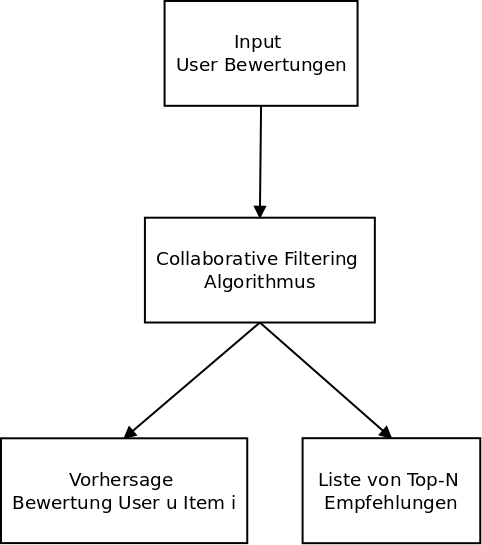
\includegraphics[width=0.5\textwidth]{cf}
  \caption{Collaborative Filtering Prozess}
  \label{fig:cfprocess}
\end{figure}

\subsubsection{Speicherbasiert Methoden vs. modellbasiert}
\label{sec:cfmodels}

Collaborative Filtering kann weiter in zwei unterschiedliche Methoden aufgeteilt werden:

\begin{description}
\item[Speicherbasiert] Bei speicherbasierten Methoden werden f"ur jeden User "ahnliche User aufgrund der gespeicherten Bewertungen gesucht. Es wird eine Nachbarschaft mit "ahnlichen User erstellt. Diese Methoden nennt man auch N"achste-Nachbarn-Methoden oder kNN-Methoden (englisch: memory-based).
"Ahnlichkeit wird aufgrund von gemeinsam bewerteten Items berechnet. Wenn zwei User f"ur mehrere Items die selben Bewertungen vergeben, sind sie sich "ahnlich. Sie haben einen "ahnlichen Geschmack. Einem User werden diejenigen Items empfohlen, die er noch nicht kennt und die eine hohe Bewertung von "ahnlichen Usern erhalten haben.
Wenn das Recommendersystem $p_{u,i}$ berechnen soll, beschafft es sich eine Liste mit allen Usern, die in der Nachbarschaft von $u$ sind und die das Item $i$ bewertet haben. Aufgrund der "Ahnlickeit zu $u$ und den vorhandenen Bewertungen der User in der Liste f"ur $i$, wird $p_{u,i}$ berechnet.
\item[Modellbasiert] Modellbasierte Methoden (englisch: model-based) nutzen die bestehenden Bewertungen um ein Modell zu erlernen. Das Modell wird auch Latent Faktor Modell genannt. User und Items werden mit Vektoren repr"asentiert. Die Elemente der Vektoren sind Pr"aferenzen und Eigenschaften.  $p_{u,i}$ wird mit den Latent Faktor Vektoren berechnet. Die Berechnung des Modells kann auf ein Optimierungsproblem reduziert werden.
\end{description}

Dieser Report beschreibt Algorithmen f"ur beide Methoden. Userbased ist speicherbasiert. Matrixfaktorisierung ist modellbasiert.

\subsection{Herausforderungen}
\label{sec:challenges}

Bei der Implementierung von Recommendersystemen ergeben sich mehrere Herausforderungen.

\begin{description}
\item[Genauigkeit]  Die Differenz zwischen $p_{u,i}$ und der tats"achlichen Bewertung soll m"oglichst klein sein.
\item[Skalierbarkeit] 
Collaborative Filtering muss f"ur Millionen User und Items m"oglich sein. Die Technik soll also f"ur grosse Datenmengen skalieren.
\item[Sparsity] F"ur eine grosse Menge an Items gibt es in der Regel nur eine kleine Anzahl an Items, die ein User auch bewertet hat. Wenn sich keine gemeinsamen Items zwischen den Usern finden, k"onnen auch keine Nachbarschaften gebildet werden.
\end{description}

\section{Evaluation}
\label{sec:evaluation}

In diesem Report werden mehrere Algorithmen zur L"osung des Recommenderproblem beschrieben. Die Qualit"at der beschriebenen Algorithmus wird gemessen und mit den anderen Algorithmen verglichen. Dieser Abschnitt beschreibt eine Methode, um die Qualit"at der Algorithmen zu evaluieren. In den nachfolgenden Abschnitten werden die Algorithmen mit dieser Methode evaluiert und miteinader verglichen.

\subsection{Daten}
\label{sec:data}

Ein Recommenderalgorithmus ben"otigt Daten, um das Model oder die Nachbarschaften zu erstellen. F"ur die Evaluation sind ebenfalls vorhandende Bewertungen notwendig. Diese Daten liegen oft in Form einer Matrix vor. Die Zeilen rep"asentieren Items und die Kolonnen User. In den Zellen steht welche Bewertung ein User einem Item gegeben hat. Diese Matrix nennt man Ratingmatrix.

Die Daten f"ur Recommender Systeme k"onnen auf zwei unterschiedliche Arten beschafft werden.

\begin{description}
\item[Explizites Feedback] Bei explizitem Feedback verl"asst man sich auf Daten die User explizit eingegen haben. Beispielsweise werden User aufgefordert, dem System ihre Pr"aferenzen anzugeben oder man pr"asentiert den User eine Reihe von Items, die er auf einer Skala von 1 bis 5 bewerten muss. Ein Problem von explizitem Feedback ist, dass es oft zu d"unn besetzten Ratingmatrizen f"uhrt, da die User nur eine kleine Anzahl Items explizit bewerten.
\item[Implizites Feedback] Implizites Feedback leitet die Bewertungen der User f"ur Items aus Beobachtungen ab. Das System beobachtet die Interaktionen, wie zum Beispiel in Vergangenheit gekaufte Artikel, Browsehistory, Suchanfragen oder Klickverhalten, des User mit dem System. Oft besteht implizites Feedback nur aus boolschen Werten. Das heisst entweder ein Ereignis ist eingetreten oder nicht.
\end{description}

\subsubsection{MovieLens Daten}
\label{sec:movielens}

F"ur das Projekt wurden die Daten von Movielens verwendet. MovieLens wurde von vom GroupLens Projekt an der Universit"at Minnesota entwickelt. Die Daten werden mit einer Webanwendung gesammelt. User k"onnen Filme bewerten und MovieLens gibt den User darauf eine Top-N Empfehlungsliste. Die Daten k"onnen von http://www.grouplens.org/node/12 heruntergeladen werden. 

Das Datenset enth"alt die Bewertung von 943 User und 1682 Items. Die Daten sind in Kolonnen strukturiert. Die erste und zweite Kolonne enth"alt User und Item ID. Die dritte Kolonne enth"alt ein Zahl zwischen 1 und 5. Die repr"asentiert die Bewertung. Und in der vierten Kolonne ist ein Zeitstempel der Bewertung. Das Movielens Datenset enth"alt insgesamt 100000 Bewertungen. Abbildlung \ref{fig:movielens} zeigt einen Auschnitt der rohen Daten.

\begin{figure}
\centering
\begin{verbatim}
1	1	5	874965758
1	2	3	876893171
1	3	4	878542960
1	4	3	876893119
1	5	3	889751712
\end{verbatim}
\caption{Ausschnitt aus MovieLens Datensatz}
\label{fig:movielens}
\end{figure}

F"ur den Userbased Collaborative Filter Algorithmus wurden die Daten in das CSV-Format transfomiert. Die Daten wurden mit dem Pythonskript \verb|tocsv| transformiert. Das CSV-Format eignet sich bessser, weil vorhandene Softwarebibliotheken f"ur das Einlesen der Daten genutzt werden k"onnen. In diesem Projekt wurden die Daten mit Paket \verb|cassava| eingelesen.

F"ur die Matrixfaktorisierung wurden die Daten als Matrix abgespeichert. So muss das Programm nicht bei jedem Testlauf die Transformation von 100000 Bewertungen in eine Ratingmatrix vornehmen.

\subsection{Vorgehen}
\label{sec:procedure}

Die Qualit"at des Recommenderalgorithmus wird durch die Genauigkeit der Bewertungsvorhersagen bestimmt. Man misst die Differenz zwischen vorhergesagter Bewertung $p$ und tats"achlicher Bewertung $q$. 
Um die Vorhersagen zu berechnen muss man zuerst ein Modell erstellen (Training). Danach werden mit diesem Modell Vorhersagen berechnet und mit den richtigen Bewertungen verglichen (Test). Die Evaluierung wird in zwei Phasen aufgeteilt. 

\begin{enumerate}
\item Trainingsphase
\item Testphase
\end{enumerate}

\subsubsection{Trainingsphase}

In der Trainingsphase wird ein Modell aufgrund einer Menge vorhandender Bewertungen berechnet. Diese Menge nennt man das Trainingsset. Die Funktion \verb|model| nimmt als Argument das Trainingsset und gibt als Wert ein Modell zur"uck. Dieses Modell wird in der Trainingsphase der \verb|predict|-Funktion als Argument "ubergeben. 

Bei Userbased Collaborative Filtering ist das Modell die Nachbarschaft jedes User. Bei Matrixfaktorisierung sind die Latent Faktor Vektoren das Modell.

\subsubsection{Testphase}
In der Testphase werden die Vorhersagen berechnet und mit den tats"achlichen Bewertungen verglichen. Die \verb|predict|-Funktion nimmt das Modell, einen User $u$ und ein Item $i$ als Argumente und gibt als Wert die approximierte Bewertung  $p$ zur"uck.

Um die Genauigkeit zu bestimmen, werden alle User-Item Paare aus einer Menge vorhandener Bewertungen mit der Funktion \verb|predict| auf die approximierte Bewertung $p$ abgebildet. Die Menge der vorhandenen Bewertungen nennt man Testset. Sie unterscheidet sich vom Trainingset.

\subsubsection{Evaluationsmetrik}
\label{sec:evaluationmetrik}

Es gibt verschieden Evaluationsmetriken. In diesem Projekt wurde die Metrik Mean Absolute Error ($MAE$) verwendet. Sie wird f"ur die Evaluation von Recommendersystemen h"aufig verwendet \cite{sarwar01}. Der Mean Absolute Error berechnet sich wie folgt:

Von allen approximierten Werten $p$ wird die Differenz zur tats"achlichen Bewertung $q$ berechnet. Die Abweichungen vom tats"achlichen Wert nennt man Residuen. Von der Differenz wird der Betrag berechnet. Die Abweichungen werden summiert. Schliesslich bestimmt man die mittlere Abweichung, indem man durch Anzahl Bewertungen $N$ im Testset teilt 

\begin{equation}
  \label{eq:mae}
  MAE = \frac{\sum_{i+1}^N | p_i-q_i | }{N}
\end{equation}

In diesem Projekt wurde das Set in 80000 Bewertungen f"ur die Trainingsphase und 20000 Bewertungen f"ur die Evaluierung aufgeteilt.

Abbildung \ref{fig:crossvalidation} stellt das Vorgehen der Evaluation grafisch dar.

\begin{figure}
  \centering
      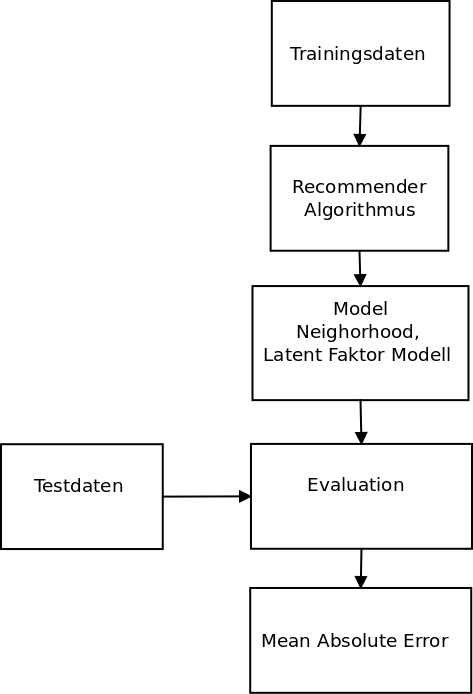
\includegraphics[width=0.5\textwidth]{evaluation}
  \caption{Evaluation}
  \label{fig:crossvalidation}
\end{figure}

\subsection{Hardware Plattform}
\label{platform}

Die Experimente wurden auf einem PC-Notebook durchgef"uhrt. Das Notebook hat 8GB Ram und die CPU ist mit 2.9Ghz getaktet.

\begin{center}
\begin{tabular}{ll}
 Prozessor        &  i7-3520M            \\
 Clock            &  2.90GHz             \\
 Arbeitsspeicher  &  8 GB                \\
 Betriebssystem   &  Ubuntu 14.04.1 LTS  \\
\end{tabular}
\end{center}

\section{Unpers"onliche Empfehlungstechniken}
\label{sec:simple}

Dieser Abschnitt beschreibt einfache, alternative, M"oglichkeiten relative gute Empfehlungen zu generieren. Diese Techniken werden in den nachfolgenden Abschnitten als Baselinealgorithmus verwendet um zu "uberpr"ufen, ob die beschriebenen Algorithmen einen tieferen MAE-Wert erreichen. So ist einfach ersichtlich, ob die Collaborative Filtering Algorithmen einen qualitativen Vorteil bringen.

Um einem User Items zu empfehlen werden oft einfache Statistiken berechnet. Diese Methoden sind unpers"onlich. Das heisst die Top-N Empfehlungen sind nicht vom pers"onlichem Geschmack von $u$ abh"angig. Jeder User erh"alt die selben Empfehlungen. 

Diese Technik wird in vielen Bereichen angewendet. Restaurantf"uhrer oder Filmkritikwebseiten erstellen oft Ranglisten, welche Restaurants oder Filme von allen Usern im Durchschnitt am besten bewertet werden. Items mit den h"ochsten Durchschnittswerten, werden dem User empfohlen \cite{jannach11}.

Die einfachste Methode eine unbekannte Bewertung $p_{u,i}$ abzusch"atzen, ist den Durschnitt aller Bewertungen zu berechnen.

\begin{equation}
  \label{eq:avg}
  p_{u,i} = \mu
\end{equation}

Wenn diese Methode wie in Abschnitt \ref{sec:procedure} evaluiert wird, erh"alt man einen MAE von 0.968. Dieser Wert kann noch weiter minimiert werden.

Bestimmte User vergeben durchschnittlich tiefere Bewertungen. Diese Tendenz $b_u$ kann man f"ur jeden User berechnen. Man berechnet die Abweichung der Bewertungen des Users $u$ vom Erwartungswert $\mu$.

\begin{equation}
  b_u = \frac{1}{|I_u|}\sum_{i \in I_u}(r_{u,i} - \mu)
\end{equation}

Die Menge $I_u$ beinhaltet alle Items, die der User $u$ bewertet hat. $r_{u,i}$ ist die Bewertung die User $u$ Item $i$ gegeben hat.

Die Abweichung $b_u$ wird bei der Vorhersage zu $\mu$ addiert, um bei der Evaluation einen besseren MAE zu erhalten.

\begin{equation}
  \label{eq:bui}
  p_{u,i} = \mu + b_u
\end{equation}

Wenn man die Tendenz der User, Item durchschnittlich h"oher oder tiefer zu bewerten, ber"ucksichtig wie in der Gleichung \ref{eq:bui} beschrieben, kann man den MAE auf 0.8501 senken. 

Items haben ebenfalls eine Abweichung vom Durchschnitt. Bestimmte Filme k"onnen tendenziel eine h"ohere Bewertung von allen Usern erhalten. Es kann also noch die Abweichung $bi$ jedes Items berechnet werden.

\begin{equation}
  \label{eq:bi}
  b_i = \frac{1}{|U_i|}\sum_{u \in U_i}(r_{u,i} - b_u - \mu)
\end{equation}

Diese Abweichung addiert man zur Vorhersage $b_{ui}$.

\begin{equation}
  \label{eq:baseline}
  p_{u,i} = \mu + b_u + b_i
\end{equation}

Wenn man die statistischen Abweichungen der einzelnen User und Items bei der Vorhersage einer Bewertung $b_{ui}$ wie in Gleichung \ref{eq:baseline} ber"ucksichtig, erreicht man einen MAE von 0.76814.

$p_{ui}$ kann relativ einfach aufgrund der vergangen Bewertungen berechnet werden.

In Abbildung \ref{fig:maebaselines} werden die verschiedenen, unpers"onlichen Recommender miteinander verglichen. 

\begin{figure}
  \centering
\begin{tikzpicture}
  \begin{axis}[
    xbar, xmin=0,
    width=12cm, enlarge y limits=0.5,
    symbolic y coords = {Globaler Durchschnitt,mit Usertendenz $b_u$, mit User-/Itemtendenz},
    xlabel={MeanAbsoluteError},
    ytick = data,
    nodes near coords, nodes near coords align={horizontal},
    ]
    \addplot coordinates {(0.968,Globaler Durchschnitt) (0.8501,mit Usertendenz $b_u$) (0.76814,mit User-/Itemtendenz)};
  \end{axis}
\end{tikzpicture}
  
  \caption{Vergleich: unpers"onliche Empfehlungen}
  \label{fig:maebaselines}
\end{figure}


\section{Userbased Collaborative Filtering}

Die Technik Userbased Collaborative Filtering ist auch als k-NN (n"achste-Nachbarn) oder speicherbasiertes Collaborative Filtering bekannt. Der GroupLens Usenet Articel Recommender verwendete als einer der ersten Recommender Systeme Userbased Collaborative Filtering. Ringo Music Recommender und der Bell Core Video Recommender verwenden auch Userbased CF \cite{ekstrand11}.

Userbased Collaborative Filtering kann in zwei Schritte aufgeteilt werden. 

\begin{description}
\item[Nachbarschaft bestimmen] F"ur jeden User $u$ wird eine Nachbarschaft $U_u$ erstellt. Diese Nachbarschaft $U_u$ enth"alt Tupel mit allen anderen Usern und deren "Ahnlichkeit $sim$ zu $u$. Die Nachbarschaft wird aufgrund der Trainingsdaten erstellt. Sie stellt das Modell von Userbased Collaborative Filtering dar. Wenn im zweiten Schritt eine unbekannte Bewertung abgesch"atzt wird, wird auf die vorberechneten Nachbarschaften zugegriffen.
\item [gewichtetes Mittel bilden] Aus $U_u$ bildet man f"ur ein Item $i$ und User $u$ eine Menge $N \subseteq U_u$. $N$ erf"ullt folgende Anforderungen. $N$ enth"alt $k$ Elemente. $N$ enth"alt nur User $u'$ die Item $i$ bewertet haben. $N$ ist aufsteigend nach der "Ahnlichkeit $sim(u,u')$ sortiert. F"ur alle User $u' \in N$, multipliziert man die Bewertung von User $u'$ mit dem Wert der "Ahnlichkeit $sim(u,u')$. Alle Produkte werden summiert und normiert. Dadurch werden Bewertungen von User, die sehr "ahnlich sind st"arker gewichtet. 
\end{description}

Userbased Collaborative Filtering sucht nach User, die "ahnlich wie der aktive User $u$ sind. Um das Modell zu erstellen, werden die vergangene Bewertungen der User verwendet.

\subsection{Informelles Beispiel}
\label{sec:example}

Bespielsweise m"ochte man die Bewertung von User Peter f"ur den Film Titanic, den Peter noch nicht bewertet hat, vorhersagen. Man sucht nach anderen Usern, die Filme "ahnlich bewerten wie Peter. Dazu beschaft man sich f"ur jeden anderen User eine Liste aller Filme, die Peter und der andere User bewertet haben. So findet man heraus, welche $k$ User Peter am "ahnlichsten sind. Das ist seine Nachbarschaft $N$. Um vorherzusagen, welche Bewertung Peter Titanic gibt, verwendet man die Bewertungen f"ur Titanic der User in $N$. Wenn "ahnliche User Titanic eine hohe Bewertung geben, wird eine hohe Bewertung von Peter vorhergesagt. Die Bewertung von Usern, die Peter sehr "ahnlich sind, haben ein gr"osseres Gewicht als die Bewertungen von Usern, die Peter un"ahnlich sind.


\subsection{Nachbarschaft bestimmen}
\label{sec:neigborhood}

Dieser Abschnitt beschreibt, wie die Nachbarschaft  $N \subseteq U$ eines einzelnen Users $u$ erstellt wird. Eine Nachbarschaft ist eine sortierte Liste von Usern. Sie ist nach der "Ahnlichkeit $sim(u,v)$ sortiert.  Der Wert $sim(u,v)$ ist ein Modell der "Ahnlichkeit zwischen dem aktiven User und einem anderen User $v$. Zuerst wird beschrieben, wie $sim(u,v)$ definiert werden kann.

Es gibt mehrere M"oglichkeiten die "Ahnlichkeit zwischen zwei User zu evaluieren. In diesem Report werden zwei Metriken beschrieben

\begin{itemize}
  \item Pearson Korrelation 
  \item euklidische Distanz
\end{itemize}

Es ist nur m"oglich die "Ahnlichkeit zwischen zwei User zu berechnen, wenn beide User ein oder mehrere Items gemeinsam bewertet haben. Wenn es keine gemeinsamen Items gibt, k"onnen die nachfolgenden Methoden nicht angewendet werden. Der Recommender wurde so implementiert, dass User, die keine gemeinsamen Items haben einen "Ahnlichkeitswert von 0 haben. Das heisst, dass die Bewertungen dieser User keinen Einfluss auf die Berechnung von $p_{u,i}$ haben. 

Listing \ref{lst:shareditems} zeigt, wie sich das Programm eine Liste aller gemeinsamen Items beschafft. Die Funktion \verb|shareditems| nimmt zwei User und eine MultiMap und gibt alle gemeinsamen Items zur"uck. Die Multimap bildet User $u$ auf Items $I_u$ ab.

\begin{lstlisting}[caption=Implementation von shareditems, label=lst:shareditems]
shareditems :: User -> User -> Multimap User Item -> [Items]
shareditems u1 u2 m = shared (lookup u1 m) (lookup u2 m)
  where shared l1 l2 = [x| x <- l1, y <- l2, x == y]
\end{lstlisting}

\subsubsection{Pearson Korrelation}
\label{sec:pearsoncorrelation}

Gem"ass \cite{jannach11} eignet sich die sogennante Pearson Korrelation gut f"ur Userbased CF. Die Pearsonkorrelation, oder Korrelationskoeffizient ist ein dimensionsloses Mass f"ur den linearen Zusammenhang von zwei Listen. Der Korrelationskoeffizient nimmt Werte zwischen -1 und +1 an. +1 bedeutet, dass die Listen sehr "ahnlich sind. -1 bedeutet dass sie un"ahnlich sind. Bei 0 besteht kein Zusammenhang. Die Pearson Korrelation ist folgendermassen definiert.

\begin{equation}
\label{eq:pearson1}
 sim(u,v) = \frac{cov(X,Y}{\sigma_X \sigma_Y} 
\end{equation}
oder
\begin{equation}
  \label{eq:pearson}
  sim(u,v)  = \frac{\sum_{i \in I_u \cap I_v}(r_{u,i} - \bar{r}_u)(r_{v,i} - \bar{r}_v)}{\sqrt{\sum_{i \in I_u \cap I_v}( r_{v,i} - \bar{r}_v)^2}\sqrt{\sum_{i \in I_u \cap I_v}( r_{v,i} - \bar{r}_v)^2}}
\end{equation}

Die Pearson Similariy ber"ucksichtig den Umstand, dass User Items konstant tiefer oder h"oher bewerten. Zwei User, die mit den Vektoren (1,2,3,4) und (2,3,4,5) dargestellt werden, erhalten die maximale "Ahnlichkeit von 1.

Um die Pearson Korrelation zu berechnen, muss man sich zuerst die Liste $I_u \cap I_v$ mit den gemeinsam bewerteten Items beschaffen. Diese Items bildet man auf die Bewertungen der entsprechenden User ab. Listing \ref{lst:item2rating} zeigt die Implementation der Abbildung. Wenn man diese beiden Listen mit Bewertungen hat, kann man die "Ahnlichkeit berechnen.

\begin{lstlisting}[caption=Implementation: Abbildung Items zu Bewertungen, label=lst:item2rating]
import Data.MultiMap
item2rating:: [Item] -> Multimap Item Double -> [Double]
item2rating is m = map (\i -> findWithDefault 0 i m) is
\end{lstlisting}

Das Paket \verb|Math.Statistics| stellt die Funktion \verb|pearson| zur Verf"ugung um den Korrelationskoeffizenten zu berechnen.

Bei der Verwendung der Pearson Korrelation sind mehrere Schwierigkeiten bei der Evaluation aufgetreten.

\begin{description}
\item[Hohe "Ahnlichkeit bei wenig Items] Die Berechnung Pearson Korrelation zwischen zwei Usern, die nur ein Item gemeinsam bewertet haben f"uhrt zu relativ hohen "Ahnlichkeitswerten, obwohl zwei User, die nur ein gemeinsames Item haben eher un"ahnlich sind.
\item[Abweichung 0] Wenn die Bewertungen eines Users f"ur alle gemeinsame Items  $I_u \cap I_v$ gleich sind f"uhrt das zu einer Standardabweichung von 0. Da in diesem Fall der Nenner in Gleichung \ref{eq:pearson1} 0 wird, ist der Korrelationskoeffizient nicht definiert, wenn ein User alle gemeinsamen Items gleich bewertet.
\item[Nur ein gemeinsamens Item] Wenn  $I_u \cap I_v$ nur ein gemeinsames Item enth"alt ist die Standardabweichung immer 0.
\end{description}

In einem ersten Versuch wurden, die oben genannten Probleme durch entsprechende Fallunterscheidung in der Implementation abgefangen. Listing \ref{lst:similarity} zeigt die Implementation.

\begin{lstlisting}[caption=Similarity, label=lst:similarity]
import Math.Statistics

similarity :: [Double] -> [Double] -> Double
similarity r1 r2
  | (length r1) < 2 = 0
  | (length r2) < 2 = 0
  | stddev r1 == 0.0 = 0
  | stddev r2 == 0.0 = 0
  |  otherwise = MS.pearson r1 r2

\end{lstlisting}

Wenn die Varianz der betrachteten Bewertungen 0 ist, gibt diese Implementation einen "Ahnlichkeitswert von 0 zur"uck. 0 bedeutet, dass es keine Korrelation zwischen den beiden Usern gibt.

Diese Implementation des Userbased Collaborative Filtering hat zu einem MAE von 0.830 gef"uhrt. Der unpers"onlichen Recommender aus Abschnitt \ref{sec:simple} hat einen MAE von 0.768 erreicht. Die Anwendung der Userbased Methode hat in dieser Form zu einem h"oheren MAE gef"uhrt und ist noch verbesserungsw"urdig. 

\subsubsection{Optimierte Pearson Korrelation}
\label{sec:optpearson}

Ein Grund f"ur die Probleme ist, dass der definierte Korrelationskoeffizient aus Gleichung \ref{eq:pearson} nur die Bewertungen der gemeinsamen Items  $I_u \cap I_v$ bei der Berechnung der "Ahnlichkeit ber"ucksichtigt. Um das Problem der undefinierten Standardabweichung zu beheben, wurde der Erwartungswert $\bar{r_v}$ durch den Erwartungswert $b_u$ (siehe Abschnitt \ref{sec:simple}, Gleichung \ref{eq:bi}) ersetzt.

Statt 
\begin{equation}
  \label{eq:naiv}
  \sqrt{\sum_{i \in I_u \cap I_v}( r_{v,i} - \bar{r}_v)^2}
\end{equation}

wird die Standardabweichung wie folgt berechnet.

\begin{equation}
  \label{eq:naiv1}
  \sqrt{\sum_{i \in I_u \cap I_v}( r_{v,i} - b_u)^2}
\end{equation}

In die Gleichung \ref{eq:pearson} eingesetzt, berechnet sich die "Ahnlichkeit folgendermassen:

\begin{equation}
  \label{eq:advanced}
  sim(u,v)  = \frac{\sum_{i \in I_u \cap I_v}(r_{u,i} - b_u)(r_{v,i} - b_v)}{\sqrt{\sum_{i \in I_u \cap I_v}( r_{v,i} - b_u)^2}\sqrt{\sum_{i \in I_u \cap I_v}( r_{v,i} - b_v)^2}}
\end{equation}

Da statt der Standardabweichung $b_u$ verwendet wird, kann nicht mehr die \verb|pearson|-Funktion aus dem Statistik Paket verwendet werden. Die Funktion \verb|pearson| wurde durch eine Implementation der Gleichung \ref{eq:advanced} ersetzt.

\subsubsection{Euklidische Distanz}
\label{sec:euclid}

Der Pearson Korrelationkoeffizient ist nicht definiert, wenn die Varianz der betrachteten Bewertungen 0 ist. Deshalb wurde eine alternative "Ahnlichkeitmetrik untersucht. \cite{segaran} schl"agt vor die euklidische Distanzmetrik f"ur Usebased Collaborative Filtering zu verwenden. Die euklidische Distanz ist auch definiert, wenn die Varianz 0 ist.

Jeder User wird als Vektor dargestellt. Die Bewertungen, die der User gemacht hat, sind die Elemente des Vektor. Die euklidische Distanz berechnet den geometischen Abstand der Vektoren. F"ur zwei User $u$ und $v$ mit $n$ gemeinsamen Items, wird die euklidische Distanz $sim(u,v)$ wie folgt berechnet:

\begin{equation}
  \label{eq:euclid}
 sim(u,v) = \sum_i^n (u_i - v_i )^2
\end{equation}

Die euklidische Distanz ber"ucksichtigt nicht, dass bestimmte User permanent h"ohere Wertungen geben.

\subsection{Unbekannte Bewertung absch"atzen}
\label{sec:compp}

In diesem Abschnitt wird beschrieben, wie die Nachbarschaft von Abschnitt \ref{sec:neigborhood} genutzt werden kann, um eine unbekannte Bewertung des aktiven User $u$ f"ur ein Item $i$ vorauszusagen.

\subsubsection{Nachbarschaft $N$ abfragen}
\label{sec:generate}

M"ochte man zu User $u$ und Item $i$ eine Bewertung vorhersagen, ben"otigt man eine geeignete Nachbarschaft $N \subseteq U$. User in $N$ m"ussen das Item $i$ bewertet haben und dem User $u$ m"oglichst "ahnlich sein.

Zuerst beschafft man sich eine Liste aller anderen User und deren "Ahnlichkeitwerten $sim(u,u
')$. Aus dieser Liste filtert man diejenigen User, die das Item $i$ bewertet haben. Die gefilterte Liste wird aufsteigend nach der "Ahnlichkeit $sim(u,v)$ sortiert. Aus dieser Liste entnimmt man die $k$ ersten Elemente. Diese Liste entspricht $N$. 

In Listing \ref{lst:neighborhood} wird gezeigt, wie die Abfrage in Haskell implementiert wurde. Die Funktion \verb|neighborhood| nimmt neben dem User $u$ und dem Item $i$ noch eine Ganzahl $k$ als Parameter. $k$ bestimmt die Gr"osse der Nachbarschaft $N$, die f"ur die Vorhersage verwendet wird.

\begin{lstlisting}[caption=Funktion um die Nachbarschaft f"ur ein User und ein Item zu abzufragen, label=lst:neighborhood]
import Data.MultiMap
neihborhood :: User
            -> Item
            -> Int
            -> MultiMap User [(Similarity, User)]
            -> [User]
neihborhood u i k m = take k (reverse (sort onlyItem i u ))
  where onlyItem i = filter (hasRated i) allneighbors
        allneighbors = lookup u m
\end{lstlisting}

Bei der Berechnung von $p_{u,i}$ kann die Gr"osse der Nachbarschaft $N$ frei gew"ahlt werden. Wenn $k$ zu klein ist, werden nur wenige Bewertungen von anderen User zu Berechnung verwendet. Da $p_{u,i}$ in diesem Fall nur von wenigen anderen Usern abh"angig ist, ist es anf"allig f"ur Ausreisser. Wenn $k$ zu gross gew"ahlt wird, werden auch die Bewertungen der User, die dem aktiven User un"ahnlich sind ber"ucksichtigt. Diese Bewertungen sind f"ur den aktiven User nicht interessant. 

\subsubsection{Unbekannte Bewertung berechnen}
\label{sec:predict}

Wenn man $N$ generiert hat, kann man damit eine unbekannte Bewertung $p_{u,i}$ absch"atzen. Jeden User $u' \in N$ bildet man auf das Produkt der "Ahnlichkeit $sim(u,u')$ mit der Bewertung $r_{u',i}$ ab. Die Werte der Abbildung werden summiert. Damit man eine Zahl zwischen 1 und 5 erh"alt, wird diese Summe normiert. Die Summe wird mit der Summe aller "Ahnlichkeitswerte $\sum_{u' \in N}{|s(u,u')|}$ normiert. Gleichung \ref{eq:computeprediction} beschreibt die Berechnung von $p_{u,i}$ formel.

\begin{equation}
  \label{eq:computeprediction}
  p_{u,i} = \frac{\sum_{u' \in N}{sim(u,u') r_{u',i}}}{\sum_{u' \in N}{|s(u,u')|}}
\end{equation}

Die Implementation der Gleichung \ref{eq:computeprediction} ist in Listing \ref{lst:knnpredict} dargestellt. Die Funktion \verb|predict| nimmt User, Item, Model und $k$ als Argument. Das Model enth"alt die vorberechneten Nachbarschaften. Die Funktion \verb|knn| greift darauf zu und stellt die Nachbarschaft f"ur den aktiven User und dem gew"unschten Item zusammen.

\begin{lstlisting}[caption=Berechnung von $p_{u,i}$, label=lst:knnpredict]
  predict :: User
   -> Item
   -> Model
   -> Int
   -> Double
predict u i k m = rating / normalization
  where n = neighborhood u i k m
        normalization = sum [ s | (s,_,_) <- u i k m]
        rating = sum [s * r | (s, r, u) <- u i k m]
\end{lstlisting}

Bei der Evaluation hat sich herausgestellt, dass die Anwedung von Gleichung \ref{eq:computeprediction} zur Absch"atzung von unbekannten Bewertungen schlechte Resultate liefert. Die Methode erreichte einen MAE von 1.0514. 

Die Methode kann optimiert werden, indem man nur die Abweichung der Bewertung $r_{u,i}$ vom Mittel $\bar{r_u}$  aller Bewertungen des Users ber"ucksichtig. Die Abweichung ist

\begin{equation}
  \label{eq:dev2}
r_{u',i} - \bar{r_{u'}}
\end{equation}

Wenn man das in die Gleichung \ref{eq:computeprediction} einsetzt erh"alt man

\begin{equation}
  \label{eq:optcomputeprediction}
  p_{u,i} = \bar{r_u} + \frac{\sum_{u' \in N}{sim(u,u') (r_{u',i} - \bar{r_{u'}})}}{\sum_{u' \in N}{|s(u,u')|}}
\end{equation}

Die Resultate der optimierten Berechnung werden in Abschnitt \ref{sec:eqpredictresults} pr"asentiert.

\subsection{Resultate}
\label{sec:userbasedresults}

Userbased Collaborative Filtering nimmt drei Parameter.
\begin{itemize}
\item "Ahnlichkeitsmetrik
\item Formel f"ur Berechnung unbekannter Bewertungen $p_{i,u}$.
\item Nachbarschaftsgr"osse $k$
\end{itemize}

Mithilfe der Evaluation k"onnen experimentell diejenigen Parameter gefunden werden, die zum geringsten MAE f"uhren. In diesem Abschnitt werden die Resultate der Experimente pr"asentiert. 

\subsubsection{"Ahnlichkeitsmetrik}
\label{sec:simresults}

In Abschnitt \ref{sec:neigborhood} wurden drei "Ahnlichkeitsmetriken vorgestellt:

\begin{itemize}
\item Pearson Korrelation
\item Optimierte Pearson Korrelation
\item Euklidische Distanz
\end{itemize}

\begin{figure}
\begin{tikzpicture}
  \begin{axis}[
    xbar, xmin=0.7, xmax=0.95,
    height=6cm,width=10cm, enlarge y limits=0.5,
    symbolic y coords = {Euklidische Distanz,Pearson Korr.,Opt. Pearson Korr.},
    xlabel={Mean Absolute Error},
    ytick = data,
    nodes near coords, nodes near coords align={horizontal},
    ]
    \addplot coordinates {(0.872,Euklidische Distanz) (0.831,Pearson Korr.) (0.718,Opt. Pearson Korr.)};
  \end{axis}
\end{tikzpicture}
\centering
\caption{Vergleich der "Ahnlichkeitsmetriken euklidische Distanz und Pearson Korrelation}
\label{fig:comparesim1}
\end{figure}

Der Vegleich der "Ahnlichkeitmetriken wurde mit einer Nachbarschaftsgr"osse $k$ von 5 erstellt und $p_{i,u}$ wurde mit der Formel \ref{eq:optcomputeprediction} berechnet. Abbildung \ref{fig:comparesim1} zeigt die Resultate der Experimente.

Der Vergleich der "Ahnlichkeitsmetriken zeigt, dass der optimierten Korrelationskoeffizienten den kleinsten Fehler macht.


\subsubsection{Berechnung unbekannter Bewertungen}
\label{sec:eqpredictresults}

\begin{figure}
\begin{tikzpicture}
  \begin{axis}[
    xbar, xmin=0.7, xmax=1.1,
    height=6cm,width=10cm, enlarge y limits=0.5,
    symbolic y coords = {Bewertung,Abweichung,},
    xlabel={Mean Absolute Error},
    ytick = data,
    nodes near coords, nodes near coords align={horizontal},
    ]
    \addplot coordinates {(1.0514,Bewertung) (0.841,Abweichung)};
  \end{axis}
\end{tikzpicture}
\centering
\caption{Vergleich der Berechnungmethoden f"ur $p_{u,i}$}
\label{fig:predicteq}
\end{figure}

Eine unbekannte Bewertung kann auf mehrere Arten berechnet werden. In Abschnitt \ref{sec:predict} wurden die Formeln \ref{eq:computeprediction} und \ref{eq:optcomputeprediction} zur Berechnung  von $p_{u,i}$ beschrieben. Beide Formeln wurden mit den Testdaten evaluiert. Wie in Abbildung \ref{fig:predicteq} ersichtlich hat diese "Anderung der Berechnung einen starken Einfluss auf den MAE. Die Messungen wurden mit einer Nachbarschaftsgr"osse von 20 und dem Pearson Korrelationskoeffizienten durchgef"uhrt.


\subsubsection{Gr"osse der Nachbarschaft}
\label{sec:neighborhoodsize}

Die Gr"osse der Nachbarschaft $k$ hat grossen Einfluss auf die Qualit"at des Recommender. Um den besten Wert f"ur $k$ herauszufinden wurden mehrere Testl"aufe mit unterschiedlichem $k$ ausgef"uhrt.

\begin{figure}
  \centering
\begin{tikzpicture}
  \begin{axis}[
    title=Sensitiv"at der Nachbarschaftsgr"osse,
    xlabel=Anzahl Nachbarn,
    ylabel=MAE,
]
\addplot table {kdata.dat};
  \end{axis}
\end{tikzpicture}

\caption{Vergleich der "Ahnlichkeitsmetriken euklidische Distanz und Pearson Korrelation}
\label{fig:nrofneighbors1}
\end{figure}

Abbildung \ref{fig:nrofneighbors1} zeigt den Mean Absolute Error in Abh"angigkeit der Nachbarschaftsgr"osse $k$. F"ur das gegebene Testset funktioniert eine Nachbarschaftsgr"osse von 10 am besten.

\subsubsection{Fazit}

\begin{figure}
  \centering
\begin{tikzpicture}
  \begin{axis}[
    xbar, xmin=0.6,
    height=4.5cm, width=12cm, enlarge y limits=0.5,
    symbolic y coords = {Userbased CF,unpersoenlich},
    xlabel={MeanAbsoluteError},
    ytick = data,
    nodes near coords, nodes near coords align={horizontal},
    ]
    \addplot coordinates {(0.66,Userbased CF) (0.7681,unpersoenlich)};
  \end{axis}
\end{tikzpicture}

\caption{Vergleich von Userbased CF mit unpers"onlichen Empfehlungen}
\label{fig:uuvsbui}
\end{figure}

Die Experimente zeigen, dass die optimierte Pearson Korrelation und die Berechnung mit Abweichung mit einer Nachbarschaftsgr"osse von 10 die besten Resultate bei der Evaluation erreichen.

Abbildung \ref{fig:uuvsbui} zeigt einen Vergleich von Userbased Collaborative Filtering mit der unpers"onlichen Empfehlungstechnik aus Abschnitt \ref{sec:simple}. Mit den optimierten Parameter erzielt Userbased Collaborative Filtering einen 15\% kleineren MAE als die unpers"onliche Empfehlungstechnik.

Der Algorithmus ist intuitiv und relative einfach zu implementieren. Da er nur zwei Paramter hat ("Ahnlichkeitsmetrik, Nachbarschaftsgr"osse) kann man den Algorithmus einfach einsetzen. 

\section{Matrixfaktorisierung}
\label{sec:matrixfactorization}

Wie bereit in Abschnitt \ref{sec:cfmodels} erw"ahnt gibt es neben den speicherbasierten Methoden noch modellbasierte Methoden. Latent Faktor Modelle versuchen die Items und die User zu charakterisieren. 

Man geht davon aus Users und Items sogenannte Latent Faktors haben. Latent Faktor Vektoren repr"asentieren die Pr"aferenzen und Eigenschaften der User und der Items. Jedes Element eines Latent Faktor Vektors sagt aus, ob dem User eine bestimmte Eigenschaft wichtig ist oder nicht oder ob das Item eine bestimmte Eigenschaft hat oder nicht. 

\subsection{Intuition}
\label{sec:intuition}

Ein User der Action mag aber keine Romanze k"onnte zum Beispiel durch folgenden Vektor repr"asentiert werden.

\begin{equation}
  \label{eq:vektor}
  p_u = \left(
  \begin{array}[c]{c}
    5 \\
    1 
  \end{array}
\right)
\end{equation}

Die 5 repr"asentiert Action und die 1 repr"asentiert die den Romantik Preferenz.

 Ein Film kann ebenfalls nach den selben Dimensionen bewertet werden. Ein Vektor kann beschreiben wie actiongeladen oder wie romantisch ein Film ist. Die Bewertung ist das Skalarprodukt der Pr"aferenzen des Users und den Eigenschaften des Items. Das heisst die Bewertung ist maximal, wenn die Latent Faktor Vektoren von User $p_u$ und Item $p_i$ "ubereinstimmen.

Beim Latent Faktor Ansatz ist es nicht relevant, welche Bedeutung die Elemente in den Featurevektoren haben. Es geht nur darum die Muster zu finden. Matrixfaktorisierung berechnet Vektoren f"ur Eigenschaften, die wir gar nicht interpretieren k"onnen.

\begin{figure}
\centering
\begin{tikzpicture}[inner sep=5pt]
\begin{axis}[
  nodes near coords,
  enlargelimits=0.5,
  xlabel= Action,
  ylabel=Romantik,
  x
  ]
\addplot+[only marks,
point meta=explicit symbolic]
coordinates {
(0.5,0.3) [Braveheart]
(0.1,0.9) [Die Farbe Lila]
(0.6,0.7) [Lord of the Rings]
(0.1,0.1) [99 Francs]
(0.9,0.0) [Rambo 4]
};
\end{axis}
\end{tikzpicture}
\caption{Filme k"onnen durch Vektoren repr"asentiert werden. In diesem Modell besteht ein Film aus den Eigenschaften Action und Romantik}
\label{fig:moviedimension}
\end{figure}

Abbildung \ref{fig:moviedimension} veranschaulicht die Idee. In Abbildung \ref{fig:moviedimension} werden Filme als Objekte in einem Diagramm mit zwei Dimensionen dargestellt. In diesem Beispiel sind es die Dimensionen Action und Romantik. Die Eigenschaften werden als Zahlen von 0 bis 1 ausgedr"uckt. Rambo 4 ist beispielweise ein Film, der durch keine Romantik und viel Action charakterisiert werden kann.

\subsection{Matrixfaktorisierung Modell}
\label{sec:matrixfactorizationmodel}

Jedes Item kann durch einen Vektor $q_i \in \mathbb{R}^f$ repr"asentiert werden und jeder User kann durch einen Vektor $p_u \in \mathbb{R}^f$ repr"asentiert werden. $f$ entspricht der Anzahl Eigenschaften. Wenn man die Bewertung von Item $i$ f"ur User $u$ absch"atzen m"ochte, kann man das Vektorprodukt von $q_i$ und $p_u$ berechnen.

\begin{equation}
  \label{eq:rui}
  \hat{r_{ui}} = q_i^T p_u
\end{equation}

$\hat{r_{ui}}$ bescheibt wie gut die Pr"aferenzen des Users $u$ mit den Eigenschaften des Items $i$ "ubereinstimmen. Das nennt man die Interaktion zwischen User und Item.

In Haskell kann die Gleichung \ref{eq:rui} einfach implementiert werden. Das Modul \verb|Data.Vector| aus dem Package \verb|vector| stellt die Funktion \verb|vdot| zur Verf"ugung. Die Implemantation ist in Listing \ref{lst:rui} dargestellt.

\begin{lstlisting}[caption=Implementation der Vorhersage, label=lst:rui]
import Data.Vector
rui:: Vector -> Vector -> Double
rui qi pu = vdot qi pu
\end{lstlisting}

\subsubsection{Dimensions Reduktion}
\label{sec:dimred}

Repr"asentiert man alle m"oglichen User-Item Interaktion mit der Ratingmatix ben"otigt viel Speicher

\begin{equation}
  \label{eq:dimre1}
  \text{Anzahl Items} * \text{Anzahl User} = \text{Eint"age in der Ratingmatrix}
\end{equation}

Mit dem Movielens Datenset entspricht das

\begin{equation}
  \label{eq:dimre}
  1682 * 943 = 1586126
\end{equation}

Eintr"age. Wenn man die Interaktionen durch die Latent Faktor Vektoren mit 40 Faktoren repr"asentiert ben"otigt weniger Speicher. 

\begin{equation}
  \label{eq:dimred}
  \text{Anzahl Features}* (\text{Anzahl Items}*\text{Anzahl User}) = \text{Latent Faktor Elemente}
\end{equation}

In unserem Beispiel sind das noch

\begin{equation}
  \label{eq:dimred1}
  40(1682*943) = 105000
\end{equation}

Eintr"age. Das sind mehr als 15-mal weniger. Mit den Latent Faktor Vektoren kann man die Interaktion zwischen User und Item kompakter darstellen.

\subsection{Optimierungsproblem}
\label{sec:optim}

Das Recommenderproblem kann auf ein Optimierungsproblem reduziert werden.

Bei Matrixfaktorisierung geht es darum, die Latent Faktor Vektoren $q_i$ und $p_u$ f"ur jedes Item und jeden User abzusch"atzen. Sobald eine gute Absch"atzung der  Vektoren vorliegt, kann mit Hifle von Gleichung \ref{eq:rui} eine Vorhersage $ \hat{r_{ui}}$ der Bewertung eines Users $u$ f"ur ein Item $i$ berechnen werden. 

Die Vektoren $q_i$ und $p_u$ werden mit Hilfe des Trainingsset erlernt werden. 

F"ur eine vorhandene Bewertung $r_{ui}$ kann die Differenz zur Vorhersage $\hat{r_{ui}}$ wie folgt berechnet werden.

\begin{equation}
  \label{eq:error}
  e_{ui} = r_{ui} - q_i^T p_u
\end{equation}

$r_{ui}$ ist die tats"achliche Bewertung von User $u$ f"ur Item $i$. 
$e_{ui}$ nennt man Residuum.

Ziel des Recommendersystems ist, es $q_i \in \mathbb{R}^f$ und $p_u \in \mathbb{R}^f$ so zu w"ahlen, dass die Summe aller Fehler $e_{ui}$ minimal wird. Die Berechnung der Gleichung \ref{eq:error} f"uhrt man f"ur alle Bewertungen im Trainingsset durch und berechnet die Summe der Residuen.

\begin{equation}
\label{eq:errorsum}
  \sum_{(u,i) \in \kappa} (r_{ui} - q_i^T p_u)
\end{equation}

$\kappa$ entspricht dem Trainingsset.

Formell ausgedr"uckt lautet das Optimierungsproblem 
\begin{equation}
  \min_{q*,p*} \sum_{(u,i) \in \kappa} (r_{ui} - q_i^T p_u)
  \label{eq:objective1}
\end{equation}
.

\subsubsection{Regularisierung}
\label{sec:regularization}

Wenn man Gleichung \ref{eq:objective1} minimiert, werden $q_i$ und $p_u$ so gew"ahlt, dass der Fehler f"ur das Trainingsset minimiert wird. Das ist aber nicht gew"unschte Verhalten. Man m"ochte die Vektoren mit dem Trainingsset berechnen und sie sp"ater auf ein unbekanntes Set anwenden. Die Gleichung \ref{eq:objective1} bestimmt Parameter, die sich auf das Trainingsset spezialisieren. Die Optimierung soll also generalisiert werden.

 Dieses Verhalten wird mit einem Regularisierungterm erreicht. Der Regularisierungsterm f"uhrt dazu, dass die Elemente von $q_i$ und $p_u$ nicht zu gross werden. Die Konstante $\lambda$ kontrolliert wie stark die Gleichung \ref{eq:objective1} regularisiert wird \cite{koren2009}. Das Optimierungsproblem mit Regularisierung lautet wie folgt:

\begin{equation}
  \label{eq:optimization}
      \min_{q*,p*} \sum_{(u,i) \in \kappa} (r_{ui} - q_i^T p_u) + \lambda (\lVert q \rVert^2 + \lVert p \lVert ^2)
\end{equation}

\subsubsection{Kostenfunktion}
\label{sec:opt}

Aus der Gleichung \ref{eq:optimization} kann man eine sogenannte Kostenfunktion herleiten. Die Optimierungsverfahren ben"otigen eine Kostenfunktion $J$. Diese Funktion soll die Latent Faktor Vektoren $q_i$ und $p_u$ als Argument nehmen und die Summe der Residuen zur"uckgeben. Umso kleiner diese Summe ist, umso besser sind die Parameter gew"ahlt. Die Kostenfunktion sieht folgendermassen aus:

\begin{equation}
  \label{eq:costfunction}
  J(q_1, \dots , q_n, p_1, \dots, p_m) =  (r_{ui} - q_i^T p_u)^2 + \lambda (\lVert q \rVert^2 + \lVert p \lVert ^2)
\end{equation}

$J$ nimmt f"ur jeden User $u$ und jedes Item $i$ einen Latent Faktor Vektor $q_i \in \mathbb{R}^f$ und $p_u \mathbb{R}^f$.

\subsubsection{Initialisierung}
\label{sec:init}

Um die Kostenfunktion $J$ zu optimieren, ben"otigt man einen Startpunkt. F"ur das Optimierungproblem \label{eq:objective} haben sich Vektoren mit kleinen Werten bew"ahrt \cite{Takacs08}. 

In diesem Projekt wurden die Elemente der Latent Faktor Vektoren mit 0.1 initialisiert.

\subsubsection{Einfacher Gradientenabstieg}
\label{sec:gradientdescent}
 
Um das Minimum zu finden, kann beispielsweise das Verfahren des Gradientenabstieg angewendet werden. Dazu wird die Kostenfunktion $J$ nach $q_i$ und nach $p_u$ abgeleitet. F"ur $q_i$ lautet die Ableitung:

\begin{equation}
  \label{eq:decx1}
  \frac{ \partial J }{ \partial q_i } = \sum (q_i^T p_j - r) p_j + \lambda q_i
\end{equation}

Und f"ur die $p_i$ wird folgendermassen abgeleitet:

\begin{equation}
  \label{eq:dectheta1}
  \frac{ \partial J }{ \partial p_i } = \sum (q_i^T p_j - r) q_j + \lambda p_i
\end{equation}

Es hat sich herausgestellt, dass das Erlernen des Modell mit dem Verfahren des Gradientenabstiegs f"ur eine Ratingmatrix mit den Dimensionen 1682 x 943 zu aufw"andig ist. Sobald man mehrere Iterationen durchf"uhrt, dauert das Verfahren mehrere Stunden. Und wenn man zu wenige Iteration durchf"uhrt, werden die Parameter nicht befriedigend optimiert. Ein Durchlauf mit 10 Iterationen dauert auf der Evaluationsplattform 44 Minuten und f"uhrte zu einem MAE von 1.0235.

Die Berechnung der partiellen Ableitungen \ref{eq:decx1} und \ref{eq:dectheta1} ist aufwendig. F"ur jeden Parameter von $J$ und f"ur jede Dimension der Latent Faktor Vektoren muss "uber das ganze Trainingsset iteriert werden.

\subsection{Funk's stochastischer Gradientabstieg}
\label{sec:funksvd}

Statt des einfachen Gradient Descent wurde eine Variante der Gradient Descent Methode implementiert. Die Methode wurde von Simon Funk beschrieben \cite{funk}. Die Implementation basiert auf dieser Beschreibung.

Bei dem stochastischer Gradientenabstieg von Simon Funk (nachfolgend Funk SGD) ist die Berechnung des Gradienten weniger aufw"andig als beim einfachen Gradientenabstieg aus Abschnitt \ref{sec:gradientdescent}.

Der Fehler $e_{ui}$ f"ur eine Bewertung aus dem Trainingsset und f"ur die Parameter $q_i$ und $p_u$ berechnet sich wie folgt:

\begin{equation}
  \label{eq:error1}
  e_{ui} = r_{ui} - q_i^T p_u
\end{equation}

Wenn man diese Gleichungen partiell nach $q_i$ und $p_u$ ableitet, erh"alt man folgende Formeln

\begin{equation}
  \label{eq:devqi}
  (r_{ui} - q_i^T p_u) * p_u =  e_{ui} * p_u
\end{equation}

\begin{equation}
  \label{eq:devpu}
    (r_{ui} - q_i^T p_u) * q_i =  e_{ui} * q_i
\end{equation}

Bei der Methode Funk SGD passt man jeden Parameter in entgegengesetzter Richtung der Ableitung an. So wird der Fehler minimiert. Die Parameter werden also wie folgt angepasst:

\begin{equation}
  \label{eq:assignpi}
 q_i \leftarrow q_i + \alpha (e_{ui} * p_u)
\end{equation}

und

\begin{equation}
  \label{eq:assignqu}
 p_u \leftarrow p_u + \alpha (e_{ui} * q_i)
\end{equation}

$\alpha$ ist eine Konstante. Sie bestimmt mit welcher Schrittweite die Paramter angepasst werden. In Abschnitt \label{sec:results} wird die Optimierung von $\alpha$ beschrieben.

Diese Aktualisierung wird f"ur alle Bewertungen im Trainingsset durchgef"uhrt. Die Aktualisierung f"ur alle Bewertungen im Trainingsset entspricht einer Iteration.

\subsubsection{Regularisierung}
\label{sec:regularization2}

In Abschnitt \ref{sec:regularization} wurde bereits beschrieben, dass es n"otig ist das Optimierungsverfahren zu regularisieren. Deshalb werden die Zuweisungen \ref{eq:assignpi} und \ref{eq:assignqu} mit einem Regularisierungsterm erweitert.

\begin{equation}
  \label{eq:assign2}
  q_i \leftarrow q_i + \alpha (e_{iu} p_u + \lambda q_i)
\end{equation}

\begin{equation}
  \label{eq:assign3}
    p_u \leftarrow p_u + \alpha (e_{iu} q_iu + \lambda p_u)
\end{equation}

$\lambda$ ist eine Konstante. Sie steuert die Regularisierung. 

\subsubsection{Implementation}
\label{sec:sgdimpl}

Listing \ref{lst:step} zeigt die Implementation der Berechnung bei jedem Aktualisierungsschritt in Haskell.

\begin{lstlisting}[caption=Berechnung eines Featurevektors, label={lst:step}]
import Data.Vector 
newqi :: Vector Double
  -> Vector Double
  -> Double
  -> Vector Double
newqi qi pu e = qi + alpha (e * pu - (lambda * pi))
\end{lstlisting}

Da die Datenstrukturen in Haskell immutable sind, k"onnen die Vektoren $q_i$ und $p_u$ beim Aktualiserungsschritt nicht einfach durch die neuen Werte ausgetauscht werden. Die Datenstruktur, die die Vektoren zusammenfasst, muss bei jedem Updateschritt neu erstellt werden. Dieser Umstand hat bei den ersten Implementation zur Lauftzeit oft eine Out-of-Memory-Exception ausgel"ost. Das Problem kann behoben werden, indem Maps als Datenstrukturen eingesetzt werden. Die Maps werden bei jeder Iteration neu aufgebaut. Das heisst, es werden keine Updates auf die Datenstruktur ausgef"uhrt sondern nur Inserts. Diese k"onnen in O(log n) ausgef"uhrt werden und ein Teil alten Datenstruktur kann wiederverwendet werden. Listing \ref{lst:sgd} zeigt die Implementation eines Aktualisierungsschitt.

\begin{lstlisting}[caption=Implementation Funk SGD, label=lst:sgd] 
train :: Features
      -> (Int,Int) 
      -> M.Matrix Double 
      -> Features
train (x, theta) (i, u) y
  = (updateRow i newqi x, updateRow u newpu theta)
  where newqi = newqi oldqi oldpu error
        newpu = newpu oldpu oldqi error
        oldqi = M.lookup i 1 x
        oldpu = M.lookup u 1 theta
        error = eui2 (rui (i,u) y) oldqi oldpu  
\end{lstlisting}

\subsection{Resultate}
\label{sec:matrixfactorresults}

Das Verfahren Matrixfaktorisierung mit Hilfe der Funk SGD Methode nimmt vier Parameter.

\begin{itemize}
\item Anzahl Iterationen
\item Anzahl der Features $f$ der Latent Faktor Vektoren
\item Schrittweite des Gradientenabstieg $alpha$
\item Regularisierungskonstante $\lambda$
\end{itemize}

Mithilfe der Evaluation k"onnen experimentell diejenigen Parameter gefunden werden, die zum geringsten MAE f"uhren. In diesem Abschnitt werden die Resultate der Experimente pr"asentiert. 

F"ur jeden Parameter wurde ein Experiment durchgef"uhrt.

\subsubsection{Anzahl Iterationen}

Wenn die Latent Faktor Vektoren mit 0.1 initialisiert werden, erreicht die Implementation bei 200 Interationen einen MAE von 0.7544. Der MAE verbessert sich nach 200 Iterationen nur noch wenig.

\begin{figure}
  \centering
\begin{tikzpicture}
  \begin{axis}[
    title=Minimierung von $J$,
    xlabel=Anzahl Iteration,
]
\addplot table {it.dat};
  \end{axis}
\end{tikzpicture}
\caption{Wert der Kostenfunktion $J$ in Abh"angigkeit der Anzahl Iterationen mit $\alpha$ = 0.15, $f$ = 5, und $\lambda=0.01$}
\label{fig:itercostj}
\end{figure}

Abbildung \ref{fig:itercostj} zeigt den Wert der Kostenfunktion $J$ in Abh"angigkeit der Anzahl Iterationen. Der Wert der Kostenfunktion ist proportional zum MAE.

\subsubsection{Anzahl Features $f$}p

Die Anzahl Features $f$ bestimmt die Dimension der Vektoren $q_i$ und $p_u$.

\begin{figure}
  \centering
\begin{tikzpicture}
  \begin{axis}[
    title=Sensitiv"at von $f$,
    xlabel=$f$,
    ylabel=MAE,
]
\addplot table {f.dat};
  \end{axis}
\end{tikzpicture}
\caption{Sensitivit"at von $f$ mit $\alpha$ = 0.15 20 Iterationen und $\lambda=0.01$}
\label{fig:sensf}
\end{figure}

Abbildung \ref{fig:sensf} zeigt den MAE in Abh"angigkeit von $f$. Bei dieser Evaluation wurde die Anzahl Iterationen auf 20 gesetzt und $\alpha$ auf 0.15. Die Regularisierungskonstante $\lambda$ ist 0.01.

Bei dem gegebenen Datenset hat eine Dimension $f$ von 5 zum kleinsten MAE bei der Evaluation gef"uhrt.

\begin{figure}
  \centering
\begin{tikzpicture}
  \begin{axis}[
    title=Sensitiv"at von $\lambda$,
    xlabel=$\lambda$,
    ylabel=MAE,
]
\addplot table {lambda.data};
  \end{axis}
\end{tikzpicture}
\caption{Sensitivit"at von $\lambda$ mit $\alpha$ = 0.15 20 Iterationen und $f = 5$}
\label{fig:lambda}
\end{figure}

\subsubsection{Regularisierungskonstante $\lambda$}

Abbildung \ref{fig:lambda} zeigt den MAE in Abh"angigkeit von der Regularisierungskonstante $\lambda$. Wenn $\lambda$ 0.01 ist, ist der MAE am kleinsten.

\subsubsection{Fazit}

Folgende Parameter haben f"ur das MovieLens Datenset zum kleinsten MAE bei der Evaluation gef"uhrt.

\begin{center}
\begin{tabular}{lr}
 Parameter           &  Wert  \\
 $\lambda$              &  0.02  \\
 Anzahl Iterationen  &    200  \\
 $alpha$             &  0.15 \\
\end{tabular}
\end{center}

\begin{figure}
\begin{tikzpicture}
  \begin{axis}[
    xbar, xmin=0,
    width=12cm,height=6cm, enlarge y limits=0.5,
    symbolic y coords = {Bias,Userbased,Matrixfaktorisierung},
    xlabel={MeanAbsoluteError},
    ytick = data,
    nodes near coords, nodes near coords align={horizontal},
    ]
    \addplot coordinates {(0.7681,Bias) (0.66,Userbased) (0.7544,Matrixfaktorisierung)};
  \end{axis}
\end{tikzpicture}
\centering
\caption{Vergleich von unpers"onlichen Empfehlungen, Userbased Collaborative Filtering und Matrixfaktorisierung}
\label{fig:compare}
\end{figure}

Abbildung \ref{fig:compare} zeigt einen Vergleich der vorgestellten Algorithmen. Bias bezeichnet die unpers"onliche Empfehlungstechnik.

\section{Implementationsdetails}
\label{sec:ram}

Dieser Abschnitt beschreibt Probleme die bei der Implementation aufgetreten sind und m"ogliche L"osungen.

F"ur den Vergleich der beschriebenen Algorithmen wurden drei Haskell-Module geschrieben. Um die Algorithmen zu Evaluieren wurde ein ausf"uhrbares Programm erstellt. Das ausf"uhrbare Programm liest die Trainingsdaten und Testdaten, erstellt ein Modell und berechnet den Mean Absolute Error und gibt diesen aus.

\subsection{Projekstruktur}
\label{sec:structur}

Das Haskell Projekt besteht aus vier Modulen. Abbildung \ref{fig:structur} zeigt die Aufteilung. Die Algorithmen wurden in den Modulen Bias, Userbased und Matrixfactorization implementiert. Diese Module stellen die beiden Funktionen \verb|predict| und \verb|model| zur Verf"ugung.

Die Funktion \verb|model| berechnet das Modell. Dieses wird an die Funktion \verb|predict| weitergegeben. \verb|predict| nimmt ausserdem einen User und ein Item als Argument und gibt als Wert Vorhersage $p_{u,i}$ der Bewertung zur"uck.

\begin{figure}
  \centering
      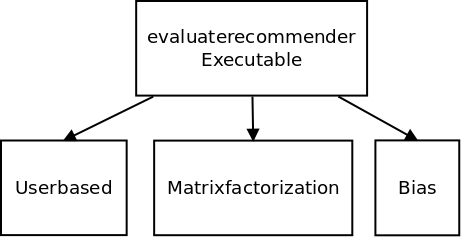
\includegraphics[width=0.5\textwidth]{structur}
  \caption{Projektstruktur}
  \label{fig:structur}
\end{figure}

\begin{description}
\item[evaluaterecommender] Dieses Modul enth"alt das ausf"uhrbare Programm. Es nutzt die Module Userbased, Matrixfactorisation und Bias um die Evaluation durchzuf"uhren. Der Programmcode f"ur die MAE Berechnung ist ebenfalls in diesem Modul enthalten.
\item[Userbased] Das Modul Userbased enth"alt den Userbased Collaborative Filtering Recommender.
\item[Matrixfactorization] Das Modul enth"alt einen Recommender der Matrixfaktorisierung nutzt.
\item[Bias] Das Modul Bias implementiert die unpers"onlichen Empfehlungstechniken.
\end{description}

\subsection{Build System}
\label{sec:cabal}

Um das Projekt zu kompilieren und die Abh"angigkeiten aufzul"osen, wurde das Buildtool Cabal eingesetzt. Die verwendete Version ist 1.20.0.2. Cabal ein Paketisierung und Build System f"ur Haskell. Cabal wird verwendet, weil die Implementation der Algorithmen Pakete aus dem Repository Hackage verwendet. Cabal l"ost Abh"angigkeiten zu Hackage Paketen automatisch auf. Ausserdem verwaltet Cabal Projektmetadaten, wie Lizenz, Author, u.s.w.

\subsubsection{Sandboxing}
\label{sec:sanboxing}

Das Projekt wurde in einer sogenannten Sandbox erstellt. Wenn das Projekt in einer Sandbox erstellt wird, werden alle Abh"angigkeiten des Projekt in einer separaten Paketverwaltung installiert. Das hat den Vorteil, dass "Anderungen an der globalen Paketverwaltung das Projekt nicht beinflussen. Der Befehl lautet:
\begin{verbatim}
cabal sandbox init
\end{verbatim}

\subsection{Daten einlesen}
\label{sec:readio}

Beim Einlesen der Daten sollte mit \verb|ByteString| gearbeitet werden. Dieser Abschnitt beschreibt, weshalb \verb|ByteString| eingesetzt wird.

Bei der Ausf"uhrung der Evaluation werden die Daten vom Filesystem eingelesen. Das Modul \verb|Prelude| bietet daf"ur die Funktion
\begin{verbatim}
readFile:: FilePath -> IO String
\end{verbatim}
 . \verb|FilePath| ist ein Alias f"ur \verb|String|. Die Funktion nimmt einen Dateipfad und gibt eine IO Action zur"uck. Die IO Action liest den Inhalt des Files und bindet Resultat an einen String.

Ein \verb|String| ist eine Liste. Listen werden in Haskell ``lazy'' evaluiert. Ein File ist f"ur Haskell also nur eine Liste von Zeichen. Wenn die Listen lazy evaluiert werden sind die Elemente darin nur ein Versprechen, dass das Element zur Verf"ugung steht, wenn es ben"otigt wird. Die Berechnung des Elements hat noch nicht stattgefunden. Das ist normalerweise kein Problem aber wenn diese Liste ein Stream von der Festplatte ist, ist das Einlesen vergleichweise langsam, weil jedes Zeichen einzeln von der Festplatte geholt wird.

Die Standardbibliothek Prelude bietet zwei Datentypen, die sich f"ur das effiziente Einlesen der Daten eignen.

\begin{itemize}
\item \verb|Data.ByteString.Strict|
\item \verb|Data.ByteString.Lazy|
\end{itemize}

 Die Strict-Version l"ost das Problem indem die ganze String in den Arbeitsspeicher eingelesen wird. \verb|Data.ByteString.Lazy| liest die ersten 64KB in den Arbeitsspeicher \cite{Lipovaca}.

Da die Trainings und Testdaten ca. 1.7MB gross sind, wurde f"ur dieses Project \verb|Data.ByteString.Strict| verwendet.

Listing \ref{lst:readio} zeigt wie Daten mit der Funktion \verb|readFile| eingelesen werden. Der ByteString wird der Funktion \verb|decode| "ubergeben. Diese gibt ein \verb|Either| zur"uck. Wenn ein Fehler beim Einlesen passiert enth"alt \verb|Either| eine Fehlermeldung. Sonst enth"alt es die gew"unschten Daten. Ein m"oglicher Fehler wird in der Funktion \verb|toVec| abgefangen.

\begin{lstlisting}[label={lst:readio},caption={Einlesen von Files mit ByteString}]
import Data.Csv
import qualified Data.Vector as V
import qualified Data.ByteString.Lazy as Bl

type Rating = (Int, Int, Double)

main = do
  c <- Bl.readFile basefile
  let csvData = decode NoHeader c
  let v = toVec csvData
  ...

toVec :: Either String (V.Vector Rating)
      -> V.Vector Rating
toVec (Left err) = error err
toVec (Right v) = v
\end{lstlisting}

\subsection{Profiling}
\label{sec:profiling}

Die ersten Implementation der Collaborative Filtering Algorithmen haben oft zu viel Arbeitsspeicher allokiert und das Programm ben"otigte zu viel Zeit. Um Probleme der Skalierbarkeit zu l"osen wurden Statistiken "uber das Verhalten der Algorithmen zur Laufzeit erstellt.

Der GHC Compiler unterst"utzt Time und Memory Profiling. Der generierte Output zeigt, wieviel Zeit und Speicher eine Funktion verursacht. Das heisst jede Funktion hat ein sogenanntes Kostencenter. Jedesmal, wenn die Funktion aufgerufen wird, werden Zeit und Memory zu den vorhandenen Werten im Kostencenter hinzugez"ahlt. Um die Werte in Kostencenter zu berechnen, generiert der Compiler zus"atzlichen Code, der die Berechnung ausf"uhrt. Die zu analysierenden Programme m"ussen also mit der entsprechenden Compiler Option kompiliert werden \cite{Mena}.

Es k"onnen nur ausf"uhrbare Dateien analysiert werden. In diesem Projekt wurde das Programm \verb|evaluaterecommender| analysiert.

Um das Profiling einzuschalten, m"ussen drei Compiler Optionen gesetzt werden. Die Optionen k"onnen im Cabalfile im ghc-options Property gesetzt werden.
\begin{verbatim}
executable evaluaterecommender
  ghc-options:	-prof -fprof-auto -rtsopts
\end{verbatim}
\begin{description}
\item[-prof] Profiling wird eingeschaltet
\item[-fprof-auto] Alle Funktionen sind Kostencenter
\item[-rtsopts] Erm"oglicht der Runtime Optionen mitzugeben
\end{description}

Alle verwendeten Pakete m"ussen mit der \verb|--enable-library-profiling|- Option kompiliert werden.

Um einen Profilingreport zu generieren, muss das Programm mit der Runtime Option \verb|-p| ausgef"uhrt werden. Runtime Optionen k"onnen auf der Kommandozeile nach dem Programmnamen zwischen \verb|+RTS| und \verb|-RTS| mitgegeben werden.  

\begin{verbatim}
$ evaluaterecommender +RTS -p -RTS
\end{verbatim}

Das Programm generiert eine Textdatei \verb|evaluaterecommender.prof|. Diese teilt die Analyse in drei Teile auf.

Im obersten wird beschrieben, wie lange die Ausf"uhrung gedauert hat und wieviel Speicher konsumiert wurde. Im zweiten Teil werden die Funktionen, die am meisten Zeit und Speicher ben"otigen mit dem prozentualen Anteil ausgelistet. Im letzen Teil wird die Aufrufabfolge der Funktionen in Form eines Baumes beschrieben.

\begin{verbatim}
Wed Dec 24 15:05 2014 Time and Allocation Profiling Report 

evaluaterecommender +RTS -p -K100M -RTS

total time  =        0.74 secs   (741 ticks @ 1000 us,
total alloc = 1,259,391,232 bytes 

COST CENTRE   MODULE  %time %alloc

error            Main     34.7   52.3
updateRow2    Main     27.1   22.1
trainingcases Main      7.8    0.6
iter          Main      5.8    7.7
predict       Main      3.6    4.2

\end{verbatim}

\section{Fazit und Ausblick}
\label{sec:fazit}

Von den eigenen Implementationen hat Userbased Collaborative Filtering den tiefsten durchschnittlichen Fehler bei der Evaluation erreicht. Im Gegensatz zu Userbased Collaborative Filtering ist Matrixfaktorisierung schwieriger zu implementieren und zu handhaben. Bei Matrixfaktorisierung mit Gradientenabstieg m"ussen 4 Parameter von Hand optimiert werden. Bei Userbased CF muss nur die Nachbarschaftsgr"osse $k$ optimiert werden.

Die Implementierung von Funk's Gradientenabstiegverfahren hat sich als schwierig erwiesen. Da bei diesem Verfahren die Parametervektoren oft aktualisiert werden, wird viel Speicher allokiert und der Garbage Collector muss andauernd aufr"aumen. Deshalb ist es sinnvoll zu pr"ufen, ob das Optimierungsverfahren ``Funks stochastischer Gradientenabstieg'' nicht durch ein Verfahren ersetzt werden kann, dass einfacher zu parallelisieren ist. Da die verwendeten Datenstrukturen unver"anderlich sind und die meisten Funktionen keinen Seiteneffekt haben, w"urde sich die Parallelisierung der Algorithmen anbieten.

Mit der Programmiersprache Haskell k"onnen die Recommender mit wenigen Zeilen Code implementiert werden. Das Package Repository Hackage bietet unter anderem Softwarebibliotheken f"ur den Umgang mit Matrizen und Vektoren. Es enth"alt auch Statistikpakete, die f"ur die Implementierung von Recommenender Systemen genutzt werden k"onnen.

\subsection{Implementationsvergleich}
\label{sec:compare}

Die Implementationen der beiden Algorithmen Userbased Collaborative Filtering und Matrixfaktorisierung wurden mit Implementationen des LensKit Tools verglichen. 

LensKit ist ein Softwarebibliothek die verschiedene Recommender Algorithmen enth"alt. Sie wurde von GroupLens Research Lab Universit"at Minnesota \cite{ekstrandlk11} entwickelt. Sie eignet sich f"ur den Vergleich, weil LensKit Implementationen von Userbased Collaborative Filtering und Matrixfaktorisierung mit Funks SGD enth"alt.

Die LensKit Implementationen wurden mit dem selben Datenset von MovieLens wie die beschriebenen Algorithmen evaluiert.

\begin{figure}
  \centering
\begin{tikzpicture}
\begin{axis}[
ybar,
enlargelimits=0.45,
legend style={at={(0.5,-0.15)},
anchor=north,legend columns=-1},
ylabel={MAE},
symbolic x coords={Userbased,Matrixfaktorisierung},
xtick=data,
ybar=5pt,% configures ‘bar shift’
bar width=9pt,
nodes near coords,
nodes near coords align={vertical},
]
\addplot coordinates {(Userbased,0.66) (Matrixfaktorisierung,0.74)};
\addplot coordinates {(Userbased,0.65) (Matrixfaktorisierung,0.63)};

\legend{eigene,LensKit}
\end{axis}
\end{tikzpicture} 
  
  \caption{Implementationsvergleich mit LensKit}
  \label{fig:compareimpl}
\end{figure}

Die LensKit Implementationen liefern in beiden F"allen einen tieferen MAE. LensKit zeigt, dass mit Matrixfaktorisierung die besten Resultate erreicht werden k"onnen. Die eigene Implementation ist noch verbessungsw"urdig.

\bibliographystyle{plain}
\bibliography{a}
\end{document}